\documentclass[10pt,a4paper]{article}
\usepackage[margin=20mm]{geometry}\usepackage[T1]{fontenc}\usepackage{lmodern,microtype,booktabs,graphicx,xcolor,hyperref,tcolorbox,parskip}
\setlength{\emergencystretch}{3em}
\definecolor{ink}{HTML}{172B4D}\definecolor{teal}{HTML}{167C80}\definecolor{mist}{HTML}{F1F6F8}
\hypersetup{colorlinks=true,linkcolor=teal,urlcolor=teal}
\title{\vspace{-2em}\color{ink}\bfseries Training-data uncertainty in IDM-Viz\\[.2em]\large NOAA moving-block refit sensitivity}
\author{Phase 3 supplementary experiment}\date{17 November 2026}
\begin{document}\maketitle\vspace{-1em}
\begin{tcolorbox}[colback=mist,colframe=teal,boxrule=0pt,leftrule=2mm]\textbf{Scope.} This estimates sensitivity to historical training rows by refitting the frozen pipeline on 200 moving-block bootstrap draws. It does not provide a generalization guarantee or make the NOAA same-day task a forecast.
\end{tcolorbox}
\section*{Protocol}
The chronological training partition contains 3642{} processed rows. Each bootstrap replicate resamples contiguous blocks of 30{} processed rows to the original training length. For every draw we refit the training scaler, logistic classifier, PCA anchor and clusters, then refit the isotonic correctness map on the fixed calibration partition and recompute reference correctness on the fixed reference partition. Calibration, reference and monitoring rows are not resampled. The same 21 complete 500-row monitoring batches are used across all refits; the trailing 426 rows remain excluded as in the original run. Monitoring outcomes are consulted only after the model scores and concern values for a draw are computed.

This is a training-only component sensitivity. It does not combine training, calibrator and reference uncertainty into one joint procedure; the separate 7/30/90-row block analysis for calibration/reference remains a distinct analysis.
\section*{Findings}
The mean width of the 95\% bootstrap interval for batch accuracy estimates is 0.0191. The mean width for plug-in concern is 0.0884. The accuracy-estimate bootstrap interval contains the retrospective observed batch accuracy in 2{} of 21 batches (9.5\%); this is a descriptive check on one serial stream, not a nominal-coverage claim. The mean absolute difference between the bootstrap mean estimator and observed batch accuracy is 0.0467. The refitted reference accuracy has mean bootstrap standard deviation 0.0049. Training refits changed no batch concern flags in this run (mean disagreement from the original policy: 0.000).

\begin{center}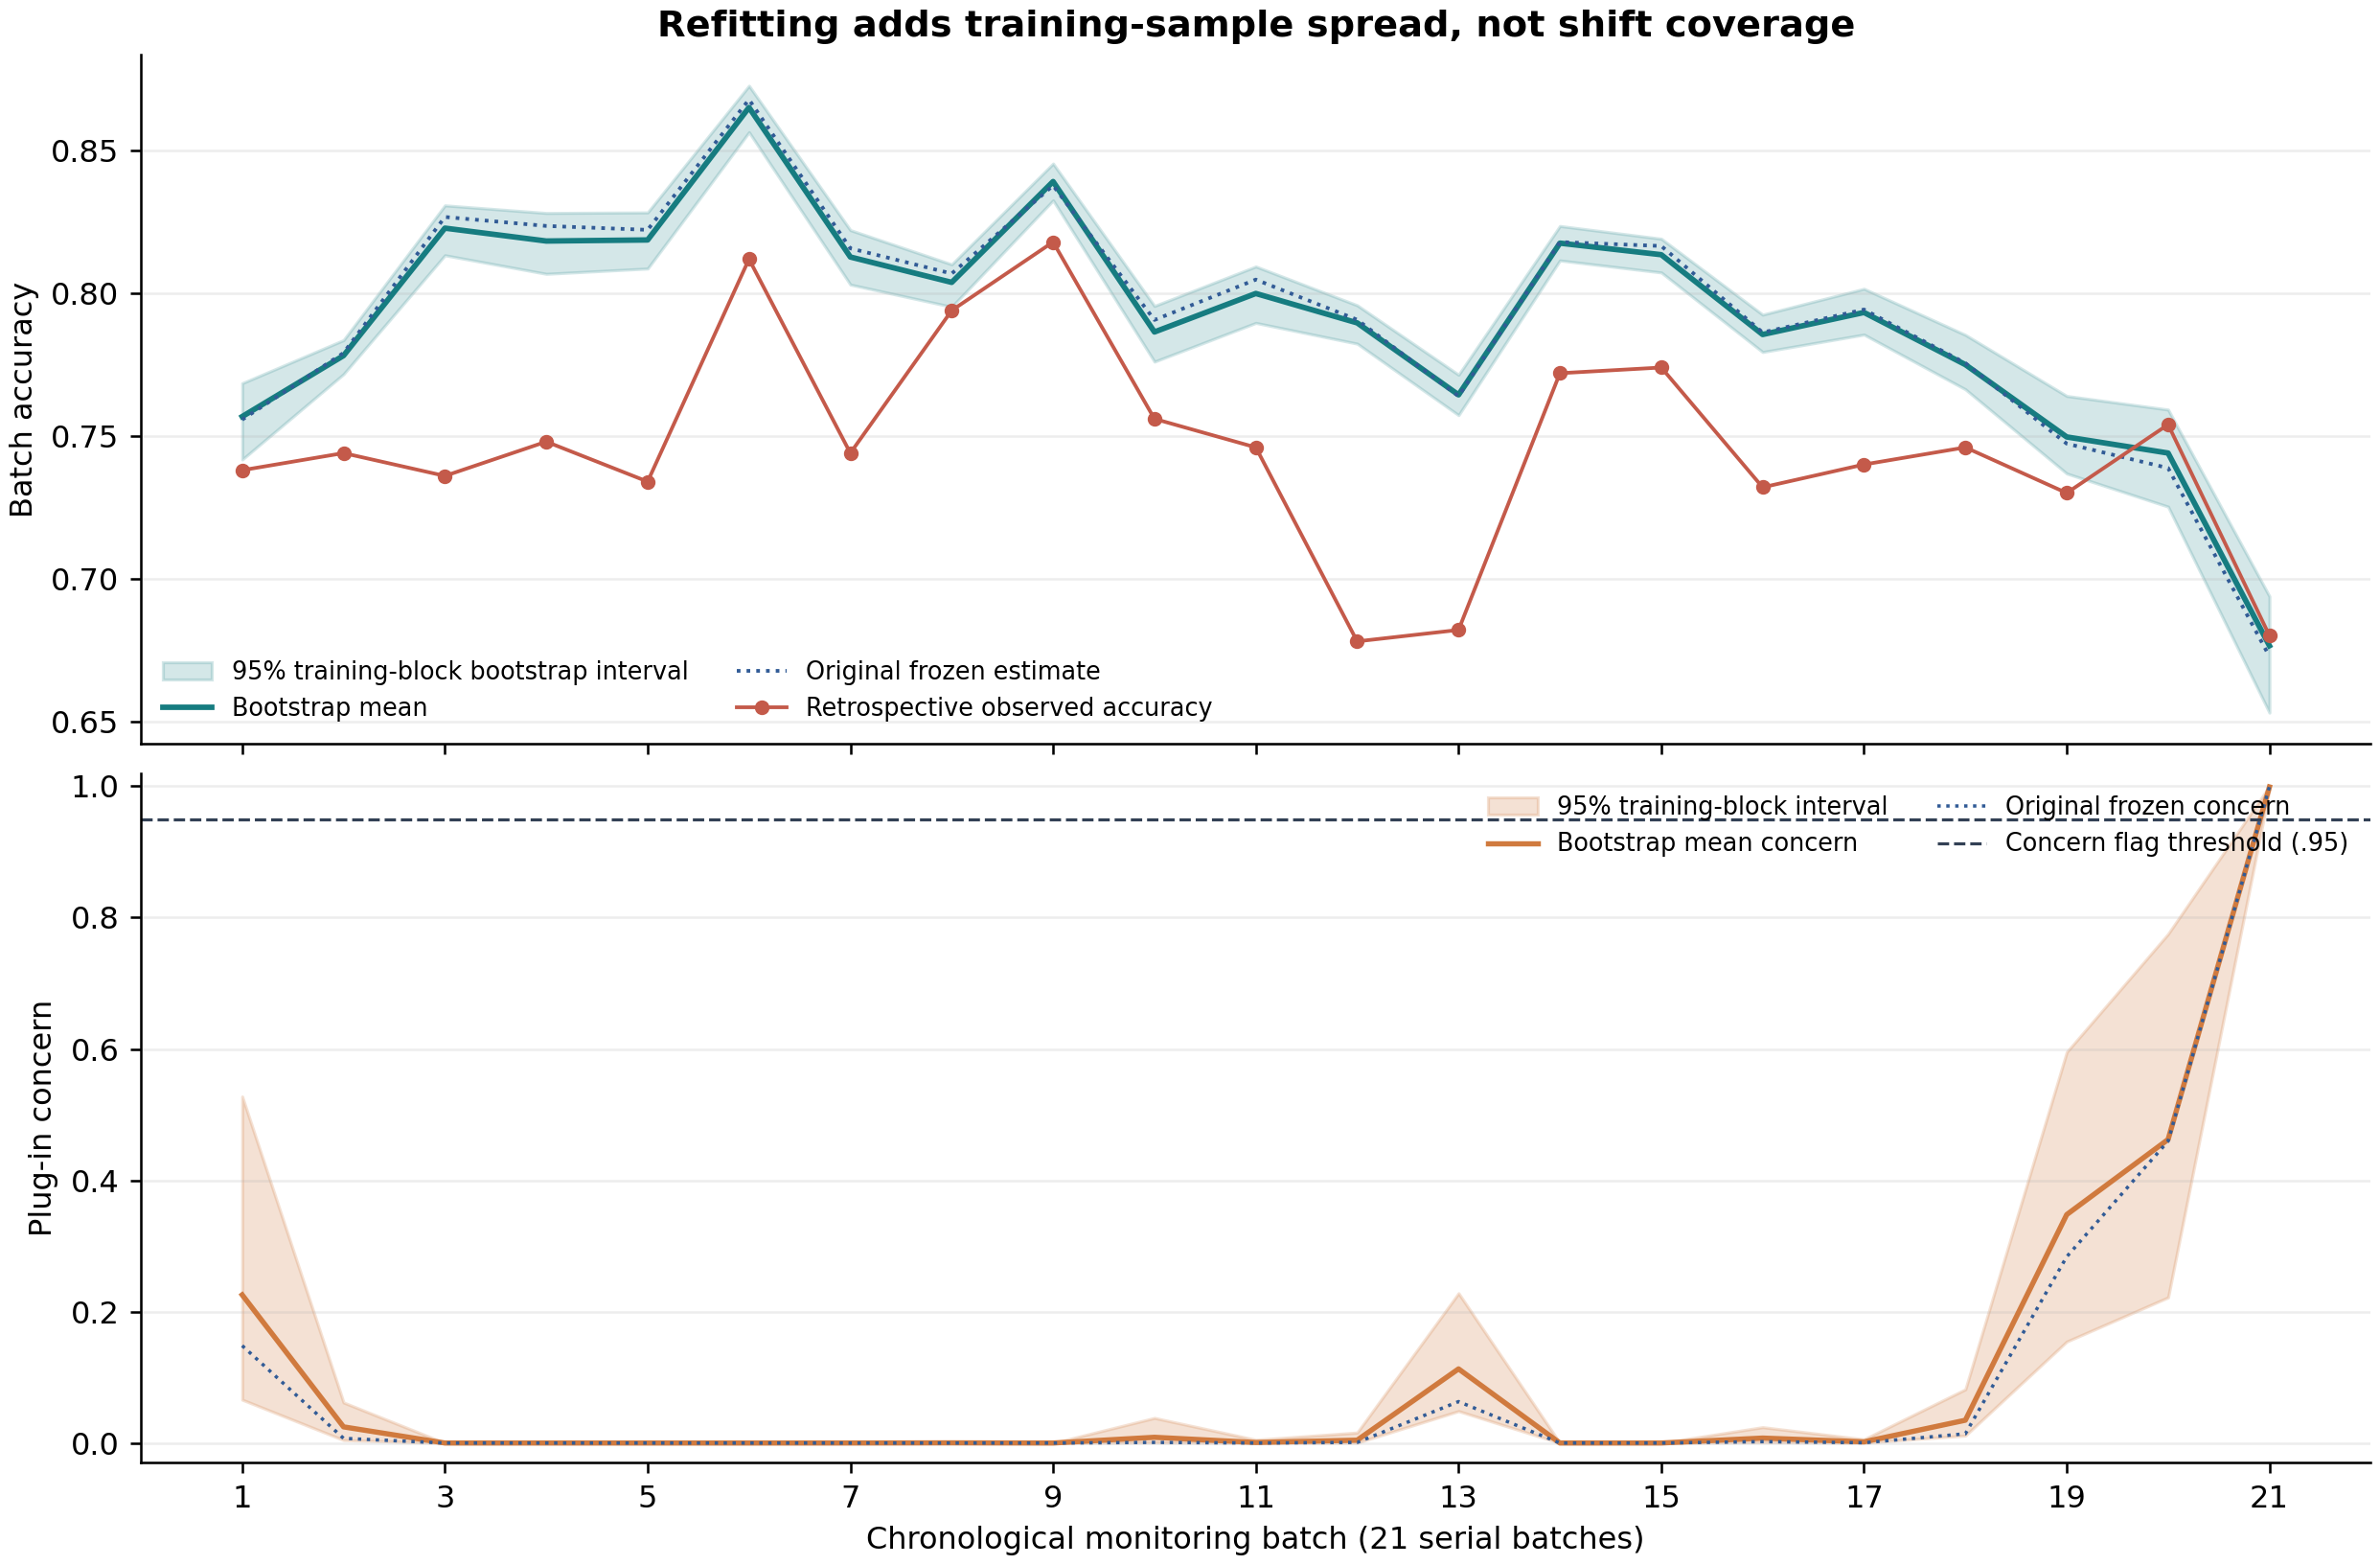
\includegraphics[width=\linewidth]{training_uncertainty.png}\end{center}
\section*{Interpretation and limits}
Retraining variability adds uncertainty to the estimated correctness and plug-in concern. However, the estimator's training-bootstrap band does not cover observed accuracy in most chronological batches, so this sensitivity analysis does not repair the NOAA transfer/calibration failure. The result is conditional on one station, a particular historical training window, a 30-row moving-block scheme, one logistic pipeline and a frozen evaluation chronology. The bootstrap cannot represent model misspecification, new-station transfer, unobserved future regimes, or arbitrary conditional shift. Block length is a design sensitivity, not an identified dependence horizon.
\section*{Reproduction}
From the project root, use fresh output directories:
\begin{verbatim}
python scripts/run_noaa_training_uncertainty.py --replicates 200 --block-length 30 \\
  --output results/phase3/noaa_training_uncertainty_cleancheck
python scripts/summarize_noaa_training_uncertainty.py \\
  --run results/phase3/noaa_training_uncertainty_cleancheck \\
  --output reports/phase3/noaa_training_uncertainty_cleancheck
\end{verbatim}
The run receipt records exact source/output hashes, bootstrap attempts, software versions and the fixed temporal partitions.
\end{document}
